%%%%%%%%%%%%%%%%%%%%%%%%%%%%%%%%%%%%%%%%%
% Tutorial
% LaTeX Template
% Version 1.0 (09/27/17)
%
% Author:
% Ben Roose (ben.roose@wichita.edu)
%
% Original template author:
% Adam Glesser (adamglesser@gmail.com)
% www.LaTeXTemplates.com
%
% License:
% CC BY-NC-SA 3.0 (http://creativecommons.org/licenses/by-nc-sa/3.0/)
%
%%%%%%%%%%%%%%%%%%%%%%%%%%%%%%%%%%%%%%%%%

\documentclass[12pt]{article}

\usepackage{graphicx} % Allow import of images
\usepackage{subcaption} % Required for side-by-side sub figures
\graphicspath{ {images/} } % Relative path to images directory
\usepackage[margin=1in]{geometry} % Required to make the margins smaller to fit more content on each page
\usepackage[linkcolor=blue]{hyperref} % Required to create hyperlinks to questions from elsewhere in the document
\hypersetup{pdfborder={0 0 0}, colorlinks=true, urlcolor=blue} % Specify a color for hyperlinks
\usepackage{todonotes} % Required for the boxes that questions appear in
\usepackage{tocloft} % Required to give customize the table of contents to display questions
\usepackage{microtype} % Slightly tweak font spacing for aesthetics
\usepackage{palatino} % Use the Palatino font

\setlength\parindent{0pt} % Removes all indentation from paragraphs

% Create and define the list of questions
\newlistof{questions}{faq}{\large FAQ for web access into cslab Linux environment}
% This creates a new table of contents-like environment that will output a file with extension .faq
\setlength\cftbeforefaqtitleskip{3em} % Adjusts the vertical space between the title and subtitle
\setlength\cftafterfaqtitleskip{1em} % Adjusts the vertical space between the subtitle and the first question
\setlength\cftparskip{.3em} % Adjusts the vertical space between questions in the list of questions

% Create the command used for questions
\newcommand{\question}[1] % This is what you will use to create a new question
{
\refstepcounter{questions} % Increases the questions counter, this can be referenced anywhere with \thequestions
%\hfill
\goodbreak
\par\noindent % Creates a new unindented paragraph
\phantomsection % Needed for hyperref compatibility with the \addcontensline command
\addcontentsline{faq}{questions}{#1} % Adds the question to the list of questions
\todo[inline, color=green!40]{\textbf{#1}} % Uses the todonotes package to create a fancy box to put the question
%\vspace{0.5em} % White space after the question before the start of the answer
}

% Uncomment the line below to get rid of the trailing dots in the table of contents
%\renewcommand{\cftdot}{}

% Uncomment the two lines below to get rid of the numbers in the table of contents
%\let\Contentsline\contentsline
%\renewcommand\contentsline[3]{\Contentsline{#1}{#2}{}}

\begin{document}

%----------------------------------------------------------------------------------------
%	TITLE AND LIST OF QUESTIONS
%----------------------------------------------------------------------------------------

\begin{center}
  \Huge{\bf \emph{EECS Tutorial: cslab Linux Environment Web Access}} % Main title
\end{center}

\listofquestions % This prints the subtitle and a list of all of your questions
\bigskip % Create a gap between list and first question
\href{https://github.com/benroose/tutorials/blob/master/cslab_tutorials/eecs_tutorial_cslab_ssh_access.pdf}{For direct SSH access into cslab see eecs\_tutorial\_cslab\_ssh\_access}

\newpage % Comment this if you would like your questions and answers to start immediately after table of questions

%----------------------------------------------------------------------------------------
%	QUESTIONS AND ANSWERS
%----------------------------------------------------------------------------------------

\question{How do I access the cslab Linux environment via a web-browser?}\label{guac_login}

\begin{enumerate}
  \item Open your favorite HTML5 compatible web-browser. To test the compatibility of your browser go to \href{https://html5test.com/}{html5test.com}
  \item In your browser go to the cslab \textit{guacamole} interface at \href{https://cslab-gateway.cs.wichita.edu/}{cslab-gateway.cs.wichita.edu}
  \item At the login screen enter your myWSU ID and password and you will be presented with the \textit{Apache Guacamole} home screen.

  \textbf{Enter your myWSU ID with only lowercase letters for the login username.}

\begin{figure}[h]
%\caption{Example of \textit{Guacamole} home screen when you first log in}
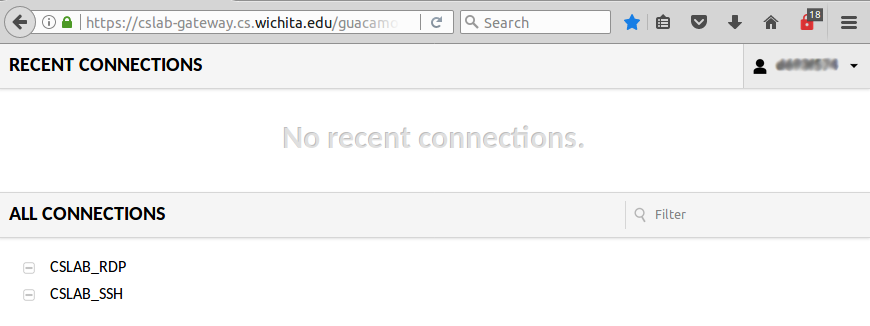
\includegraphics[width=\linewidth]{screenshot_cslab_initial_homescreen}
\centering
\end{figure}

  \item To connect into an LXDE graphical RDP desktop session for working on programming assignments click on \texttt{CSLAB\_RDP}.
  \item To connect into a command-line SSH terminal session for working on programming assignments click on \texttt{CSLAB\_SSH}.
  \item When you next log into \href{https://cslab-gateway.cs.wichita.edu/}{cslab-gateway.cs.wichita.edu} the \textit{Apache Guacamole} home screen will show clickable thumbnails of your recent connections.
  \item To log out of \textit{Guacamole} from the home screen, click on your \texttt{myWSU\_ID} at the top right. This drop-down list also enables you to open the \texttt{Settings} menu which includes displaying an on-screen keyboard for mobile devices.

\begin{figure}[h]
%\caption{Example of \textit{Guacamole} home screen with recent connection thumbnails}
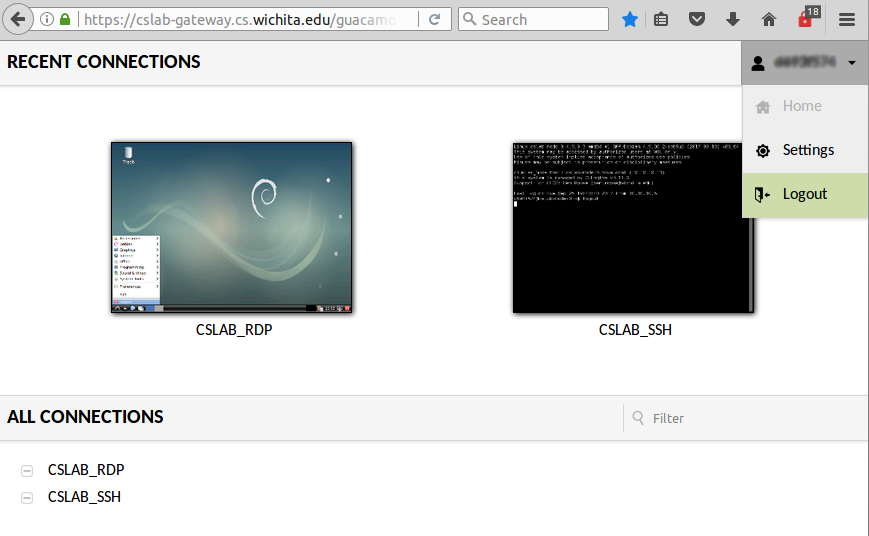
\includegraphics[width=\linewidth]{screenshot_cslab_logout_homescreen}
\centering
\end{figure}

  \item During your initial connection into an RDP desktop session, occasionally you may see a policykit error message pop-up window. This is a known software bug which is being worked on. Clicking the OK button will close the error and it should not affect the rest of your login session.
  \item To open/close the \textit{Guacamole} menu sidebar while in the cslab environment press the key combination \textbf{Ctrl+Alt+Shift}. The \textit{Guacamole} menu sidebar enables you to log out, disconnect, change settings, upload/download files, and use a remote clipboard.
  \item \textbf{When you finish your work session, please make sure to disconnect/logout from your connection within the cslab environment:
  \begin{itemize}
    \item by using the \textit{Guacamole} menu sidebar and clicking on your [username].
    \item by using the [logout] taskbar button on bottom right or [logout] menu item on bottom left within the RDP desktop session.
  \end{itemize}}
  \item \textbf{NOTE: All cslab-nodes automatically reboot every night between 2am and 3am. Any programs/processes left running will be killed during the reboot cycle.} 
  \item For further help on using the \textit{Guacamole} interface go to \href{https://guacamole.incubator.apache.org/doc/gug/using-guacamole.html}{Using Guacamole Guide}
\end{enumerate}

%------------------------------------------------

\question{What am I allowed to do within the cslab Linux environment?}\label{cslab_agreement}

\begin{itemize}
  \item You are allowed to use all software installed on the cslab Linux environment for their intended purpose of educatio and training in your programming and computer science classes at Wichita State University.
  \item When you log into the cslab environment you are accepting responsibility and accountabily for the commands, programs, and proccesses run by your Linux user account and the data stored within your user account. This is a position of trust: the university trusts that you will use cslab responsibly.
  \item If it is deemed by your instructor or the EECS systems administrator that commands, programs, or processes have been used by your user account on the cslab-nodes and associated servers for malicious purposes or outside of their intended purposes, then your access into cslab may be temporarily or permanently removed and there may be additional academic consequences to your actions.
\end{itemize}

%% \bigskip

\textbf{Never share your myWSU password with other users.}

\textbf{Never attempt to use root or sudo privileged commands within cslab environment!}

%------------------------------------------------

\question{What software is available within the cslab Linux environment?}\label{cslab_software}
\begin{itemize}
  \item cslab environment gives you both graphical and command-line Linux tools for writing, compiling, and debugging your CS programming class assignments. The Linux operating system running in cslab is Debian 9 (stretch) with a default LXDE desktop and Bash shell. Software tools/packages installed on the cslab-nodes include:

  \begin{itemize}
    \item Text and code editors: leafpad, nano, vim, and emacs.
    \item Integrated development environments (IDE): atom, geany, and eclipse.
    \item Compiling tools: GNU C compiler (gcc), g++, make, java, perl, python, python-virtualenv, haskell-compiler, prolog, flex, and bison.
    \item Debugging tools: GNU debugger (gdb) and data display debugger (ddd).
    \item Latex tools: pdflatex, texlive, and texmaker.
    \item Version control tools: git and subversion.
    \item IRC clients: hexchat, weechat, and irssi.
    \item GUI terminal emulators: terminator, lxterminal, and xterm.
    \item CLI terminal multiplexers: screen and tmux.
  \end{itemize}

  \item To check if a specific software package or version is installed within the cslab-nodes, connect into the SSH terminal session or open a terminal emulator in the RDP desktop session and type:
\begin{verbatim}
apt list --installed specify_package_name_here
\end{verbatim}

  \item If a Linux software package is not installed within the cslab Linux environment which you require to complete your class assignment, then please ask your instructor whether this package can be installed for you by the EECS systems administrator.
\end{itemize}

%% \bigskip

\textbf{Do not attempt to install any software packages yourself!}

%------------------------------------------------

\question{How do I copy text within the cslab Linux environment? }\label{text_copying}

\subsection*{Copying text from your local computer to the remote environment:}
\begin{enumerate}
  \item Copy the required text to the clipboard within your local computer application using your preferred method of copying, i.e. \textbf{Ctrl+C}.
  \item Within the cslab environment in your browser, open the \textit{Guacamole} menu sidebar by pressing the key combination \textbf{Ctrl+Alt+Shift}.
  \item Paste the copied text to the remote \textit{Guacamole} [Clipboard] field using your preferred method, i.e. \textbf{Ctrl+V}.
  \item Close the \textit{Guacamole} menu sidebar by pressing the key combination \textbf{Ctrl+Alt+Shift}.
  \item Within the RDP desktop session, any text shown in the \textit{Guacamole} [Clipboard] can be pasted into a remote cslab application by normal methods, i.e. \textbf{Ctrl+V}.
  \item Within the SSH terminal session, text in the \textit{Guacamole} [Clipboard] can be pasted into the terminal by right-clicking on the browser window with your mouse or by pressing the key combination \textbf{Ctrl+Shift+V}.
\end{enumerate}

\subsection*{Copying text from the remote environment to your local computer:}
\begin{enumerate}
  \item Within the RDP desktop session, text can be cut or copied from any cslab application by normal cut/copy methods, i.e. \textbf{Ctrl+C}.
  \item Within the SSH terminal session, text to be copied is "highlighted" using the mouse.
  \item Open the \textit{Guacamole} menu sidebar by pressing the key combination \textbf{Ctrl+Alt+Shift}.
  \item The copied or "highlighted" text will appear in the remote \textit{Guacamole} [Clipboard] and can then be selected and copied to your local computer clipboard, i.e. \textbf{Ctrl+C}.
  \item Close the \textit{Guacamole} menu sidebar by pressing the key combination \textbf{Ctrl+Alt+Shift}.
\end{enumerate}

%------------------------------------------------
\break

\question{How do I download/upload files within the cslab Linux environment? }\label{file_copying}

\subsection*{Using guacctl/guacget to download a file:}
\begin{itemize}
  \item Within the \textit{guacamole} SSH terminal session, you can use the \textit{Guacamole terminal session control utility (guacctl)} for downloading files. To download a file from the SSH terminal session to your local computer via the web-browser type:
\begin{verbatim}
guacget file_to_be_downloaded
\end{verbatim}

  \item \texttt{guacget} is an alias for the command \texttt{guacctl --download}. To see all the option flags available for this command type \texttt{guacctl}.
  \item \textbf{NOTE: \texttt{guacget} only works in SSH terminal sessions. \texttt{guacget} does not work in RDP desktop sessions.}
\end{itemize}

\subsection*{Drag-and-drop to upload a file:}
\begin{itemize}
  \item You can drag-and-drop a file from your local computer onto the cslab web-browser window. This can be used in both RDP desktop and SSH terminal sessions.
  \item By default the file is uploaded into your user home directory on the remote cslab-node.
  \item You can set a custom destination directory for future uploaded files when using drag-and-drop by typing:
\begin{verbatim}
guacctl -s custom_upload_directory
\end{verbatim}
\end{itemize}

\subsection*{\textit{Guacamole} file browser to upload or download a file:}
\begin{enumerate}
  \item Open the \textit{Guacamole} menu sidebar by pressing the key combination \textbf{Ctrl+Alt+Shift}.
  \item Click on the disk drive icon under [Devices] to open a file browser of the remote cslab-node.
  \item Browse to your user home directory on the remote server. You can then browse to subdirectories within your user home. Your home directory full path on the remote cslab-node will look like the following:
\begin{verbatim}
stu##/your_myWSU_id/
\end{verbatim}
  \item If you are unsure where your home directory is located on the remote cslab-node, in a terminal or in the SSH terminal session type \texttt{pwd} to show you the full path of your present working directory.
  \item Downloads are initiated by double-clicking on any file shown, while uploads are initiated by clicking the [Upload Files] button. Clicking [Upload Files] will open a file browsing dialog where you can choose one or more files from your local computer, ultimately uploading the selected files to the directory currently displayed within the remote cslab-node file browser.
  \item Close the \textit{Guacamole} menu sidebar by pressing the key combination \textbf{Ctrl+Alt+Shift}.
\end{enumerate}

%------------------------------------------------

\question{Can I open multiple web-browser tabs/windows into the cslab Linux environment? }\label{multiple_tabs}

\begin{itemize}
  \item cslab \textit{guacamole} interface restricts RDP desktop sessions to a single connection per user. You can view the remote RDP desktop session from only one web-browser tab/window at a time. If you attempt to open more than one web-browser tab/window and connect to a second RDP desktop session, then the gateway will present an error message in the second tab.
  \item cslab textit{guacamole} interface restricts SSH terminal sessions to a maximum of four concurrent connections per user. You can open up to four web-browser tabs/windows and connect into remote SSH terminal sessions at the same time. Each open SSH terminal session tab/window will run a separate command-line shell instance on the same remote cslab-node.
  \item You can use the \texttt{tmux} or \texttt{screen} terminal multiplexer commands to run multiple command-line shells concurrently in the same SSH session tab/window.
  \item You can open one \textit{guacamole} web-browser tab/window to connect to a graphical RDP desktop session and open additional tabs/windows to connect to SSH terminal sessions concurrently. However, the \textit{Apache Guacamole} system cannot guarantee that your RDP desktop session and your SSH terminal session(s) will connect to the same remote cslab-node.
\end{itemize}

%------------------------------------------------
\break
\question{What are the currently known bugs/glitches within the cslab Linux environment?}\label{known_bugs}

Due to the cslab environment being so new, there are a few software bugs and glitches which you may see at times. Most of these bugs occur during operations that involve the new cslab environment interacting with the older CS servers and are not critical issues.

Known bugs include:
\begin{itemize}
  \item A policykit error message pops up when user first logs into a \textit{Guacamole} RDP desktop session if other users are also logged in. This is a minor bug within policykit and can be easily mitigated by clicking \textit{Okay} in the pop-up window.
  \item When the \textit{handin} command is used in the cslab environment for programming assignment submission it may produce a \texttt{segmentation fault} error. This is caused by the older 32-bit \textit{handin} program running on the cslab 64-bit processor architecture. The error is minor and does not affect submission of student assignments for grading.
\end{itemize}

\textbf{If you experience a bug or error when using the cslab Linux environment which stops you from completing your programming assignments, please inform your instructor at your earliest convenience.}

%------------------------------------------------

\end{document}
